% -*- coding: utf-8 -*-
% !TEX encoding = UTF-8 Unicode
% !TEX root =  main.tex

\chapter{Modellbasierte Implementierung der Vektorregelung}
\label{cha:regelungpmsm}

Die Einführung in das Kapitel stellt dem Leser zunächst eine grundlegende Einführung in die Simulationstechniken und dem Anwenderprogramm Simulink dar.
Simulink ist ein Programm, welches mit MATLAB gekoppelt ist, in Simulink kann der Anwender Simulationen durchführen.
Aufgrund der Komplexität von Simulink soll an dieser Stelle nicht weiter auf die Toolboxen eingeganen werden.
Somit erhalten auch Leser ohne Erfahrungen mit dem Softwarepaket, die zum weiteren Verständnis der Arbeit benötigten Grundkenntnisse.
Der Vorteil bei der Nutzung von MATLAB basiert zum einen darauf, dass die Software etablierter Quasistandard in der Industrie und an Hochschulen ist und zum anderen auf der Benutzerfreundlichkeit bei der Durchführung von Projektarbeiten \autocite{scherf2010}.
Dem versierten Anwender der Software sei geraten, diesen Abschnitt zu überspringen.

\section{Simulation von Systemen}\label{sec:simulation}

Simulationen sind heute unverzichtbar bei der Entwicklung und Optimierung von Systemen und der Erforschung von Zusammenhängen komplexer Systeme und Prozesse \autocite{brychta}.
Die meist umfangreichen Prozesse und Systeme werden dazu in Modellen nachgebildet.
Dieses Verfahren eignet sich gut zur Analyse der Systemeigenschaften.
Dabei können die eingesetzten Simulationsmittel unterschiedlich ausfallen.

\begin{enumerate}
	\item Das System wird maßstäblich oder stark vereinfacht mit den wesentlichen Komponenten aufgebaut.
	\item Das System wird durch ein anderes physikalisches Modell nachgebildet.
	\item Das System wird durch ein mathematisches Modell beschrieben.
\end{enumerate}

Bei umfangreichen Simulationen bietet es sich an, das System in \enquote{Subsysteme} zu unterteilen (s.~h.~Abbildung~\ref{fig:subsysteme}), so dass die Modellierung mit Simulink übersichtlicher wird.
Der Vorteil gegenüber der konventionellen Modellierung von umfangreichen System, ist es, dass Fehler früher erkannt und einzelne Systeme auf physikalische Richtigkeit geprüft werden können.

\begin{figure}[h!]
	\centering
	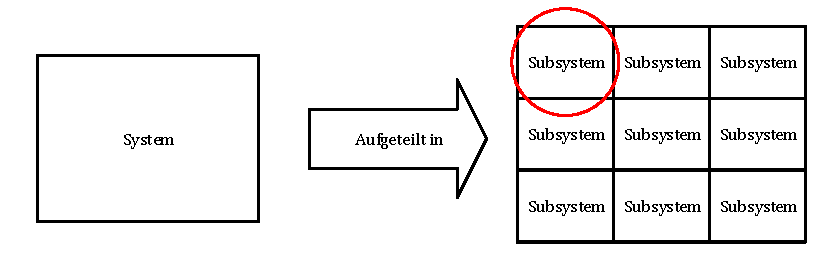
\includegraphics{/simulink/subsysteme.pdf}
	\label{fig:subsysteme}
	\caption{Semantische Abbildung zur Unterteilung eines Systemes in Subsysteme.}
\end{figure}

Das eingekreiste System kann so isoliert und gekapselt beschrieben werden.
Dazu sind die Abhängigkeiten zwischen benachbarten Subsytemen zu erfassen und bei der Kapselung geeignet zu verwerten.
Auch Subsysteme lassen sich in weitere Subsysteme zerlegen (s.~h.~Abbildung~\ref{fig:subsubsysteme}).

\begin{figure}[h!]
	\centering
	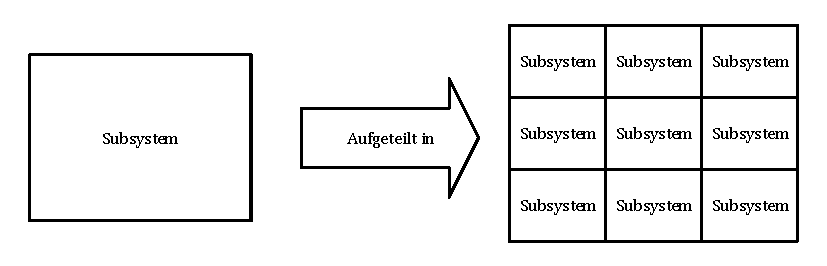
\includegraphics{/simulink/subsubsystem.pdf}
	\label{fig:subsubsysteme}
	\caption{Semantische Abbildung zur Unterteilung eines Subsystems in weitere Subsysteme.}
\end{figure}

Bei der Modellierung sollte auf die Übersichtlichkeit der Systeme geachtet werden.

\section{Einführung in Simulink}\label{sec:simulink}

MATLAB/Simulink ist vom Softwarehersteller \glqq{The Mathworks}\grqq~entwickelt worden.
Zu den Einsatzgebieten der Software zählen hauptsächlich Modellierung und Simulation technischer und physikalischer Systeme. 
MATLAB ist dabei die Kernsoftware, welche sich mit vielen Toolboxen ergänzen lässt. 
Der Name MATLAB wurde dabei von "MATrix LABoratory" abgeleitet.
Vor der Simulation eines technischen Prozesses steht die Modellbildung, welche in den vorangegangenen Kapiteln durchgeführt wurde.
Dazu sind die nötigen physikalischen Gesetzmäßigkeiten zur Beschreibung der Maschine und Regelung genutzt worden.
Als Ergebnis der Modellbildung werden nun die Differentialgleichungen, Verknüpfungen und Zusammenhänge innerhalb von Simulink zu einem geschlossen Simulationsmodell verbunden. 
Der Aufbau von den Systemen findet in Simulink mit Hilfe von Blockbildern statt, welche mit Signalflusspfeilen zu einem Signalflussplan kombiniert werden. 
Entscheidend für die Simulation von dynamischen Systemen ist die Lösung von mathematischen Zusammenhängen, insbesondere von Differentialgleichungen. 

\subsection{Simulationsbeispiel: Das mathematische Pendel}

Zur Modellbildung und Simulation eines dynamischen Fadenpendels sei zunächst die folgende Abbildung \ref{fig:pendel} gegeben:

\begin{figure}[h]
	\centering
	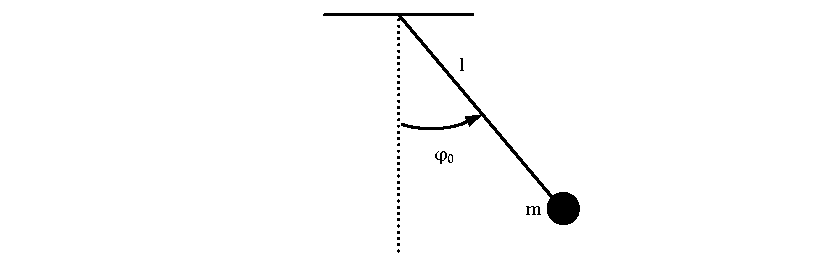
\includegraphics{/regelung/pendel.pdf}
	\label{fig:pendel}
	\caption{Fadenpendel}
\end{figure}

Er gelten folgende Momente:

\begin{center}
	\begin{tabular}{ll}
		\toprule
		Bezeichnung:				&	Mathematisches Modell: \\
		\midrule
		Rückstellmoment				&	$F_\i{Z} = m \cdot g \cdot \si{sin}(\varphi) \label{rueckstellmoment}$ \\
		Beschleunigungsmoment		&	$F_\i{B} = J \cdot \varphi = m \cdot l^{2} \cdot \ddot\varphi\label{beschleunigungsmoment} $ \\
		Reibungsmoment				&	$F_\i{R} = d \cdot l^{2} \cdot \dot\varphi\label{reibungsmoment} $ \\
		Summe aller Kräfte			&	$\sum F = 0 \label{momentengleichgewicht} $ \\
		\bottomrule 
	\end{tabular}
\end{center}

Die Bewegung des Pendels wird mit folgenden Werten simuliert:

\begin{center}
	\begin{tabular}{ll}
		\toprule
		Physikalische Bezeichnung:	& Wert: \\
		\midrule
		m		& \SI{2,3}{kg} \\
		d		& \SI{0,2}{Nms} \\
		l		& \SI{1,1}{m} \\
		g		& \SI{9,81}{m/s^2}\\
		$\varphi$ & \SI{40}{^\circ}\\
		\bottomrule
	\end{tabular}
\end{center}

Als nächster Schritt werden die physikalischen Systembeschreibungen in einer Gesamtformel zusammengefasst. 

\begin{align}
	\sum M = M_\i{R} + M_\i{B} + M_\i{Reib} = 0
	\label{momentengleichgewichtgesamt} 
\end{align}

\begin{align}
	\sum M = m \cdot g \cdot \si{sin}(\varphi) + J \cdot \varphi = m \cdot l^{2} \cdot \ddot\varphi + d \cdot l^{2} \cdot \dot\varphi = 0
	\label{momentengleichgewichtgesamt2} 
\end{align}

Wird nun die Differentialgleichung \ref{momentengleichgewichtgesamt2} nach der höchsten Ableitung $\ddot\varphi$ umgestellt, ergibt sich:

\begin{align}
	\ddot\varphi = -\dot\varphi \cdot \tfrac{\i{d}}{\i{m}} - \tfrac{\i{g}}{\i{l}} \cdot \si{sin}(\varphi)
	\label{diffgleichung} 
\end{align}

An dieser Stelle ist die Modellbildung abgeschlossen. Jetzt können die Werte in MATLAB/Simulink  verarbeitet werden.
Hier werden zuerst in der MATLAB-Umgebung Variablen mit den vorgegebenen Werten parametrisiert.

%\begin{figure}[h]
%	\centering
%	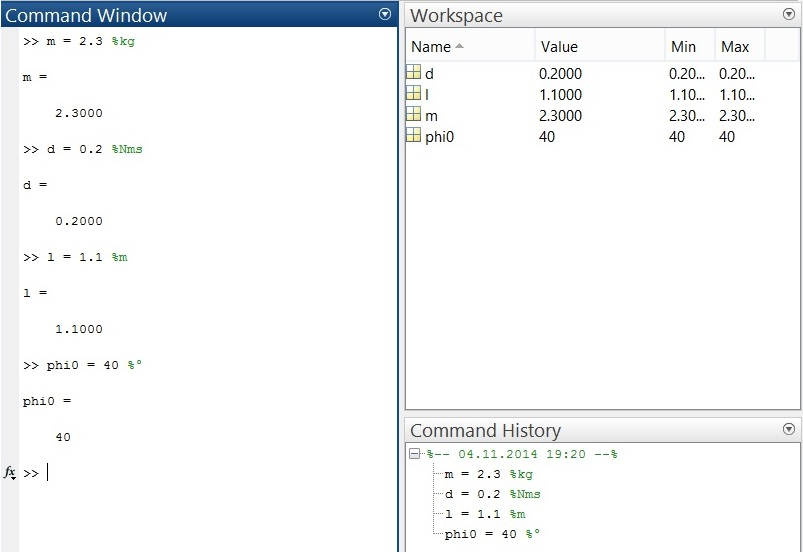
\includegraphics[width=\textwidth]{/regelung/matlab1.jpg}
%	\label{fig:matlab1}
%	\caption{Variablen in Matlab-Umgebung}
%\end{figure}

Anschließend kann in der Simulink-Umgebung das Modell entsprechend \ref{momentengleichgewichtgesamt2} aufgebaut werden.

\begin{figure}[h]
	\centering
	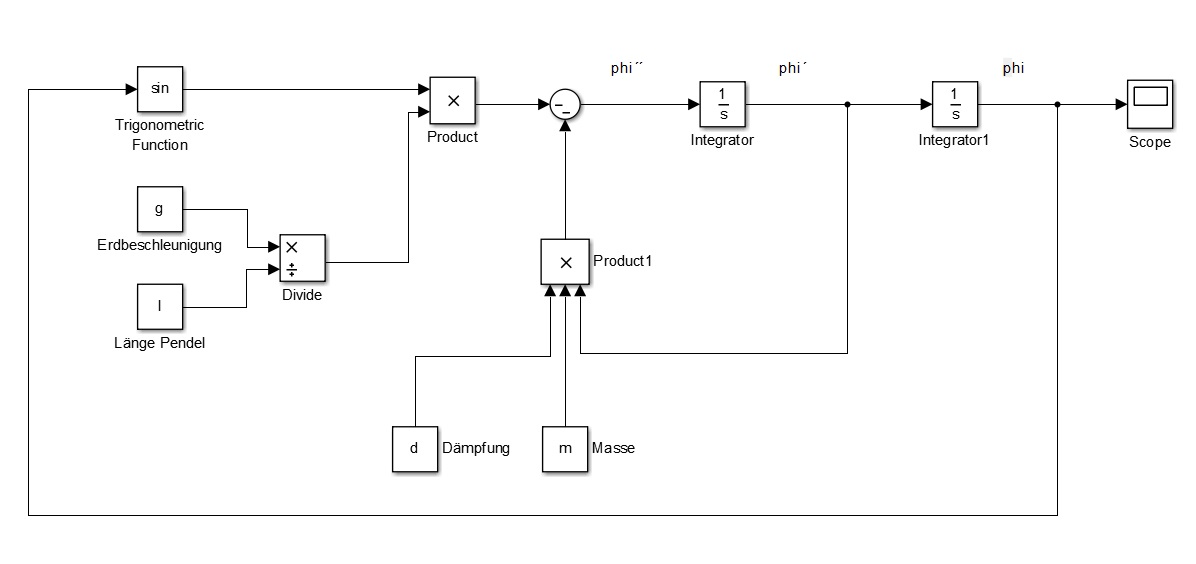
\includegraphics[width=\textwidth]{/regelung/matlab2.jpg}
	\label{fig:matlab2}
	\caption{fertiges Modell in Simulink}
\end{figure}

Mit Hilfe dieser Blöcke lassen sich  $\dot{\varphi}$ und $\varphi$ erzeugen.
Die Simulink Bibliothek bietet eine Vielzahl von mathematischen Operatoren in Form von Blockbildern.
Mit Hilfe dieser Blöcke und der Signalflusspfeile lässt sich die Gleichung in das Simulationsmodell übertragen.
Ist das Modell aufgebaut, werden die Simulationsparameter ausgewählt. 
Simulink arbeitet numerisch, daher muss ein Integrationsverfahren zur Lösung der DGLs ausgewählt werden. Voreingestellt ist das Dormand-Prince-Verfahren mit variabler Schrittweite.
Diese Methode liefert in den meisten Anwendungen gute Ergebnisse \autocite{scherf2010}.
Zur Verifizierung der Simulationsergebnisse ist es für den Anwender unumgänglich, sich im Vorfeld Gedanken zum erwartenden Ergebnis zu machen.
Im vorliegenden Beispiel sollte der Winkel $\varphi$ eine gedämpfte Schwingung in Abhängigkeit von der Zeit erzeugen.
Das Ergebnis der Simulation erhält der Anwender beim Anwählen des Blockbildes \glqq{Scope}\grqq.
%Hier zeigt sich nach durchgeführter Simulation folgendes Ergebnis:

%\begin{figure}[h!]
%	\centering
%	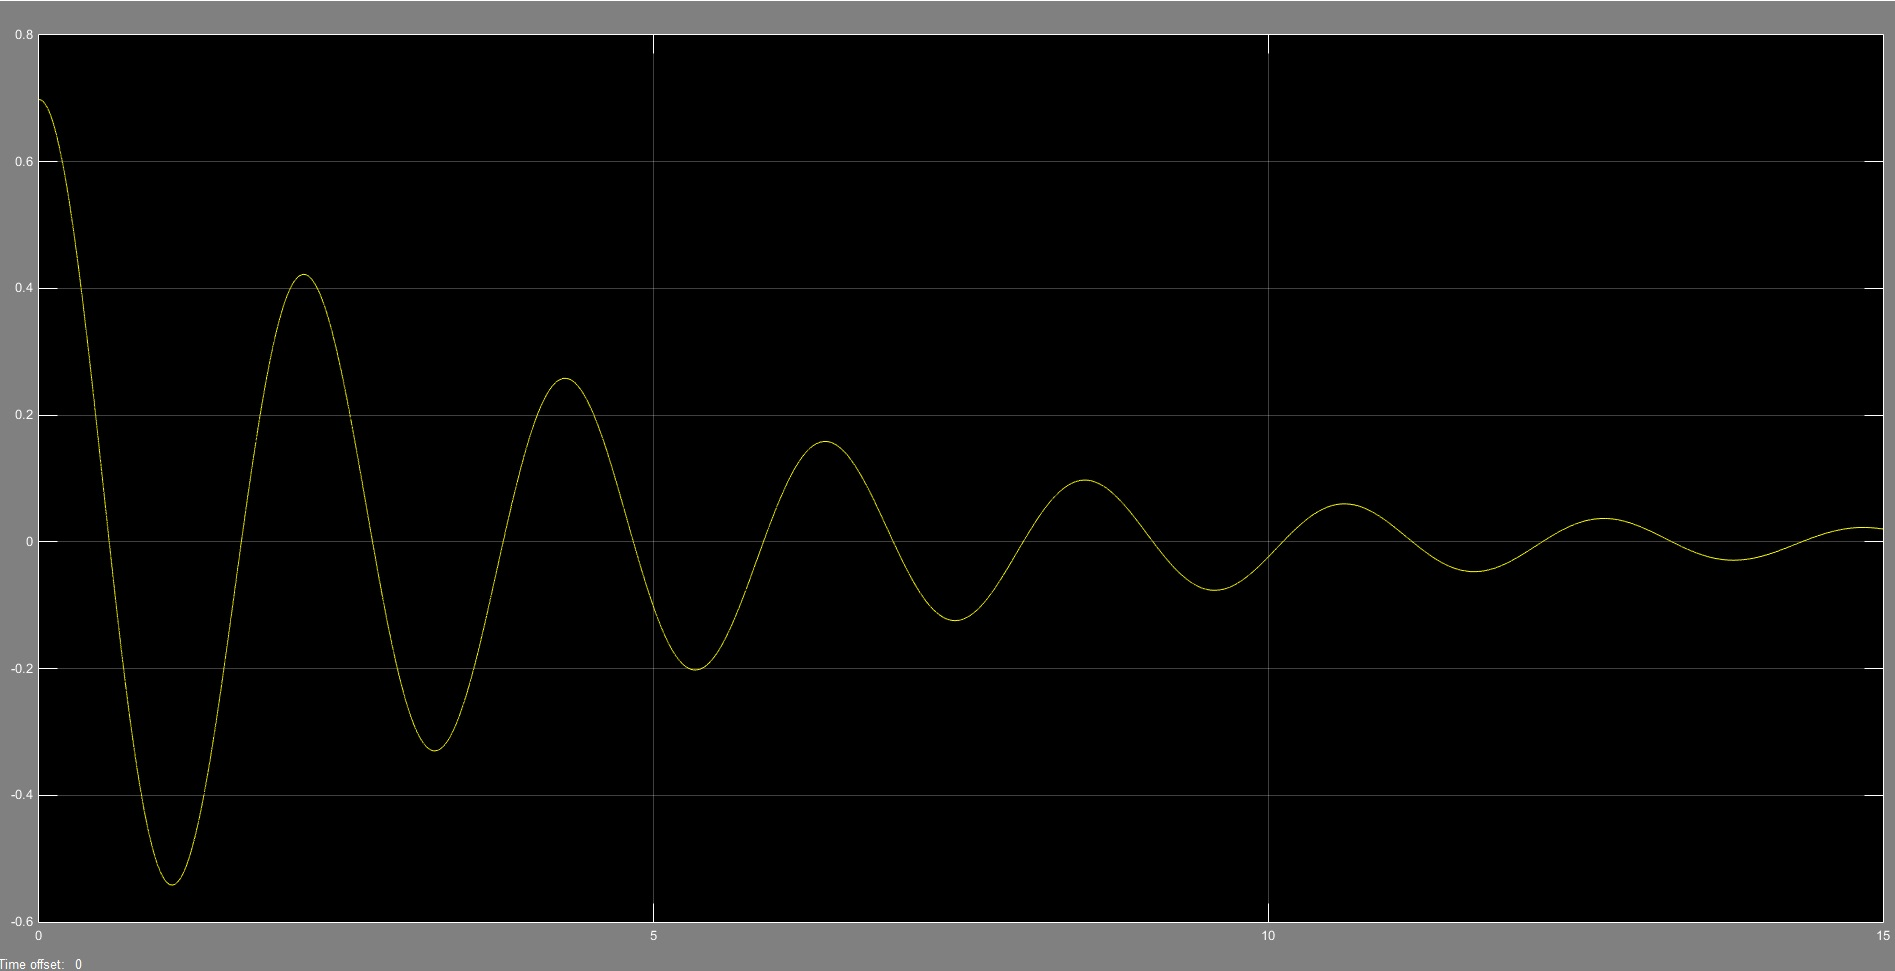
\includegraphics[width=\textwidth]{/regelung/matlab3.jpg}
%	\label{fig:matlab3}
%	\caption{Winkel $\varphi$ des Pendels über die Simulationszeit.}
%\end{figure}

%Wie erwartet, wird eine deutlich gedämpfte Schwingung des simulierten Pendels erkennbar.

\section{Simulationsblöcke}\label{sec:math-model-pmsm}

Dieses Kapitel dient zur Beschreibung der Bauteile und Komponenten, die für einen späteren Aufbau eines gesamten Regelungssystems der PMSM nötig sind.
Zunächst wird das erstellte Gesamtsystem in Abbildung \ref{fig:signalflussplan} dargestellt:

\begin{figure}[h!]
	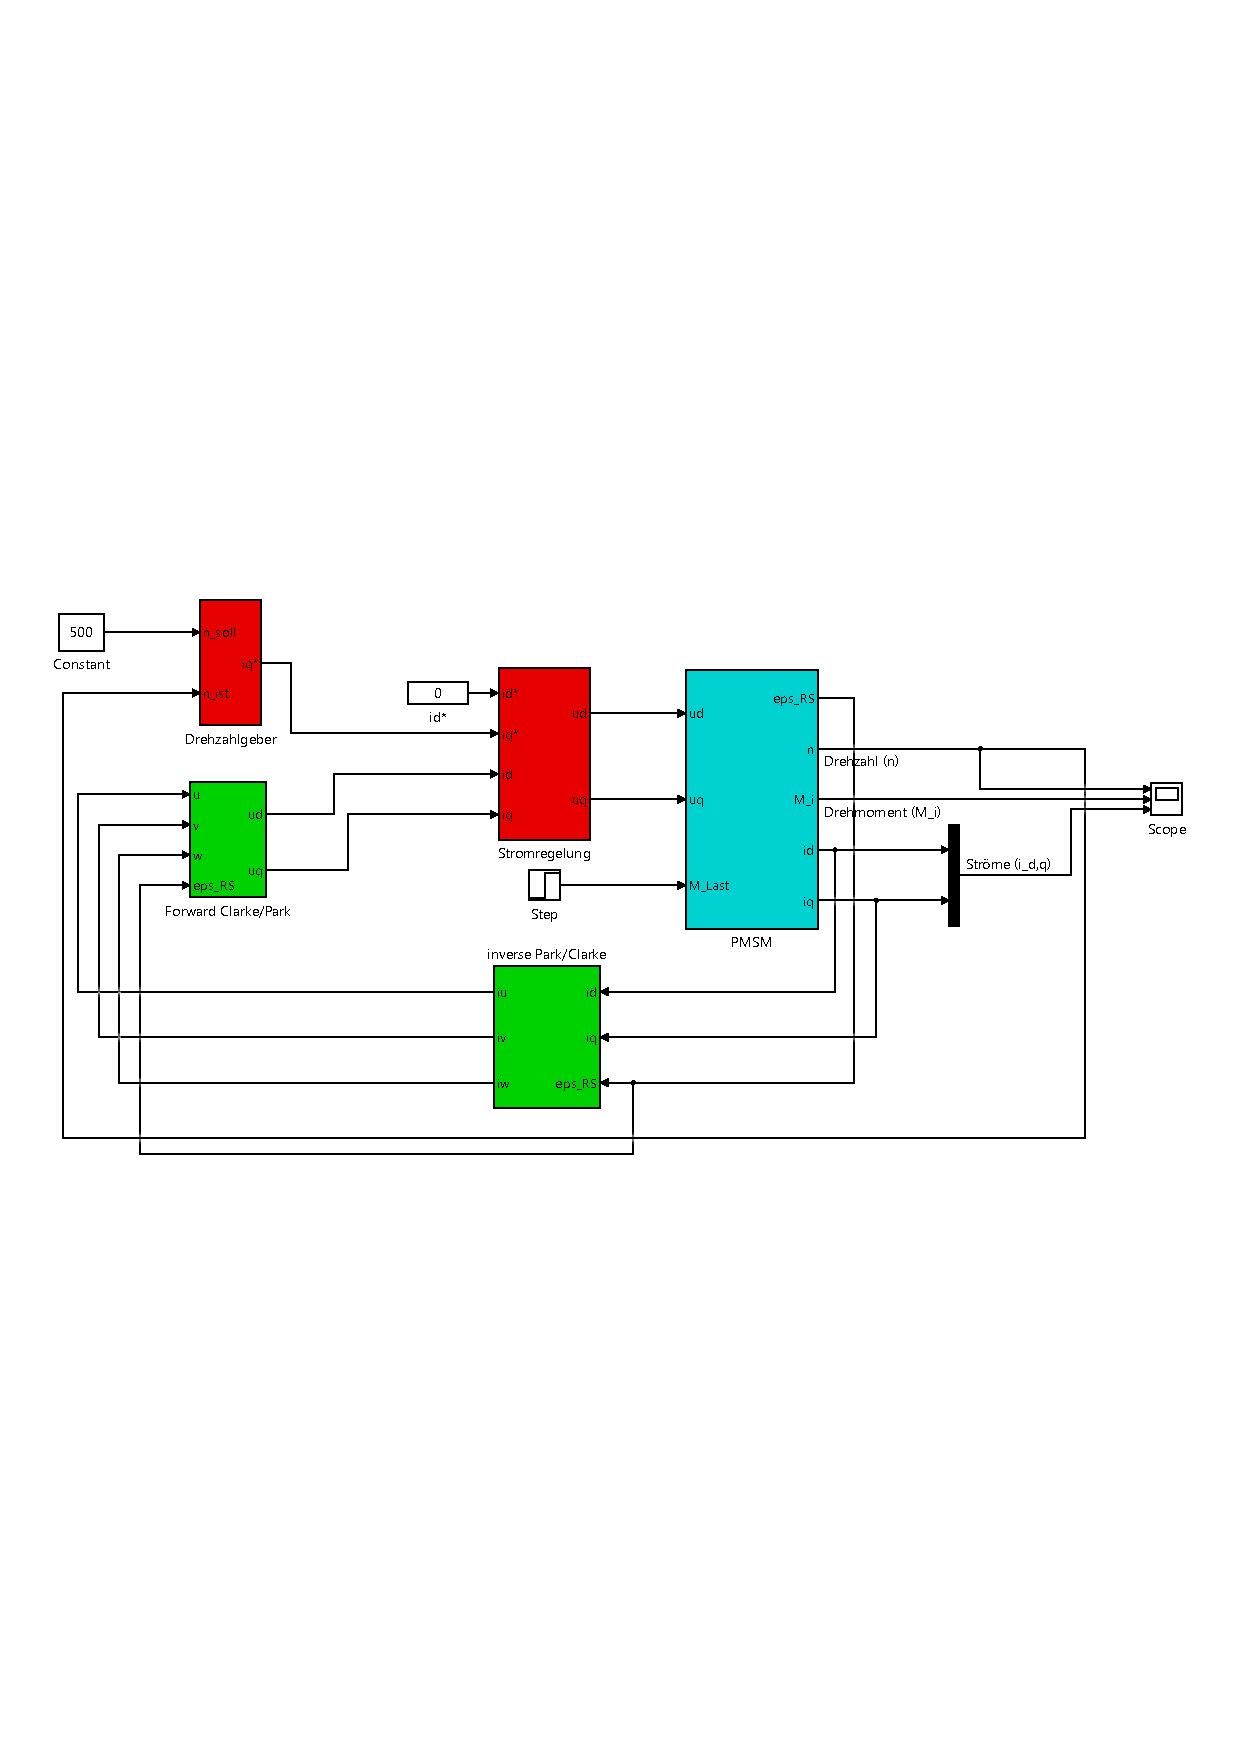
\includegraphics[width=\textwidth]{/simulink/foc-pmsm.pdf}
	\label{fig:foc-pmsm}
	\caption{Darstellung der Simulationsblöcke in Simulink.}
\end{figure}

Hier sind die Simulinkblöcke der Transformationen, das Modell der PMSM sowie Regelungskomponenten erkennbar.
Im Folgenden werden diese erläutern und deren Funktionen dargestellt.

\subsection{Transformationsblöcke}

Der Aufbau der Koordinatentransformationen leitet aus Abschnitt \ref{sec:clark} ab. 
Hierbei basiert der Block der $\alpha$-$\beta$-Transformation aus den Zusammenhängen von (\ref{clarkevektor}) und (\ref{clarkematrix}), während die Rücktransformation, die inverse $\alpha$-$\beta$-Transformation mit Hilfe von (\ref{inverseclarkevektornulleinfach}) und (\ref{inverseclarkematrixnulleinfach}) erstellt ist.
Weiterhin orientieren sich die Umsetzungen in Simulink an den Blockschaltbildern aus \ref{fig:blockbildclarkeparkkomplett} und \ref{fig:blockbildinverseclarkeparkkomplett}.

%Die folgende Abbildung \ref{fig:uvw_to_ab} zeigt den Blockaufbau der Clarke Transformation in Simulink:

%\begin{figure}[h]
%	\centering
%	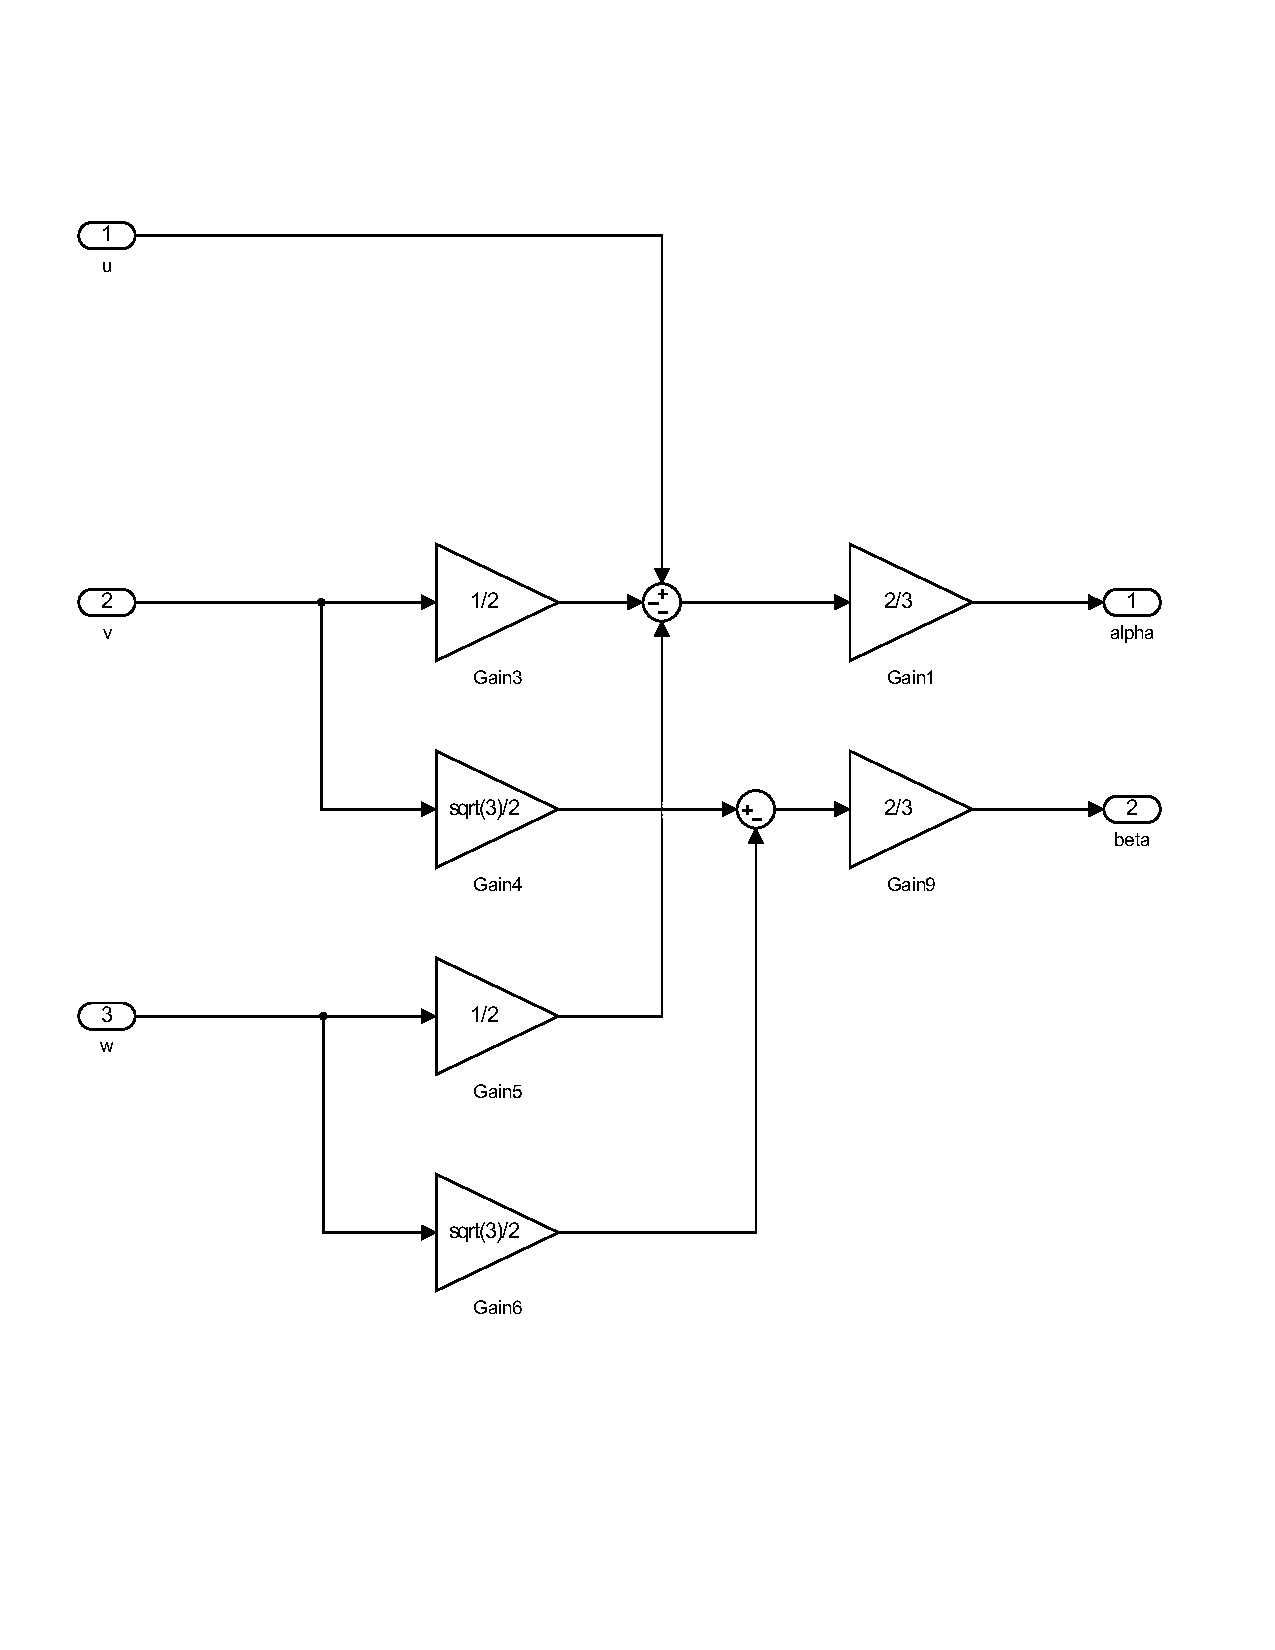
\includegraphics[width=\textwidth]{/simulink/uvw_to_ab.pdf}
%	\label{fig:uvw_to_ab}
%	\caption{Aufbau Clarke Transformation}
%\end{figure}

%In Abbildung \ref{fig:uvw_to_ab} wird der Aufbau der inversen Clarke Transformation gezeigt:

%\begin{figure}[h]
%	\centering
%	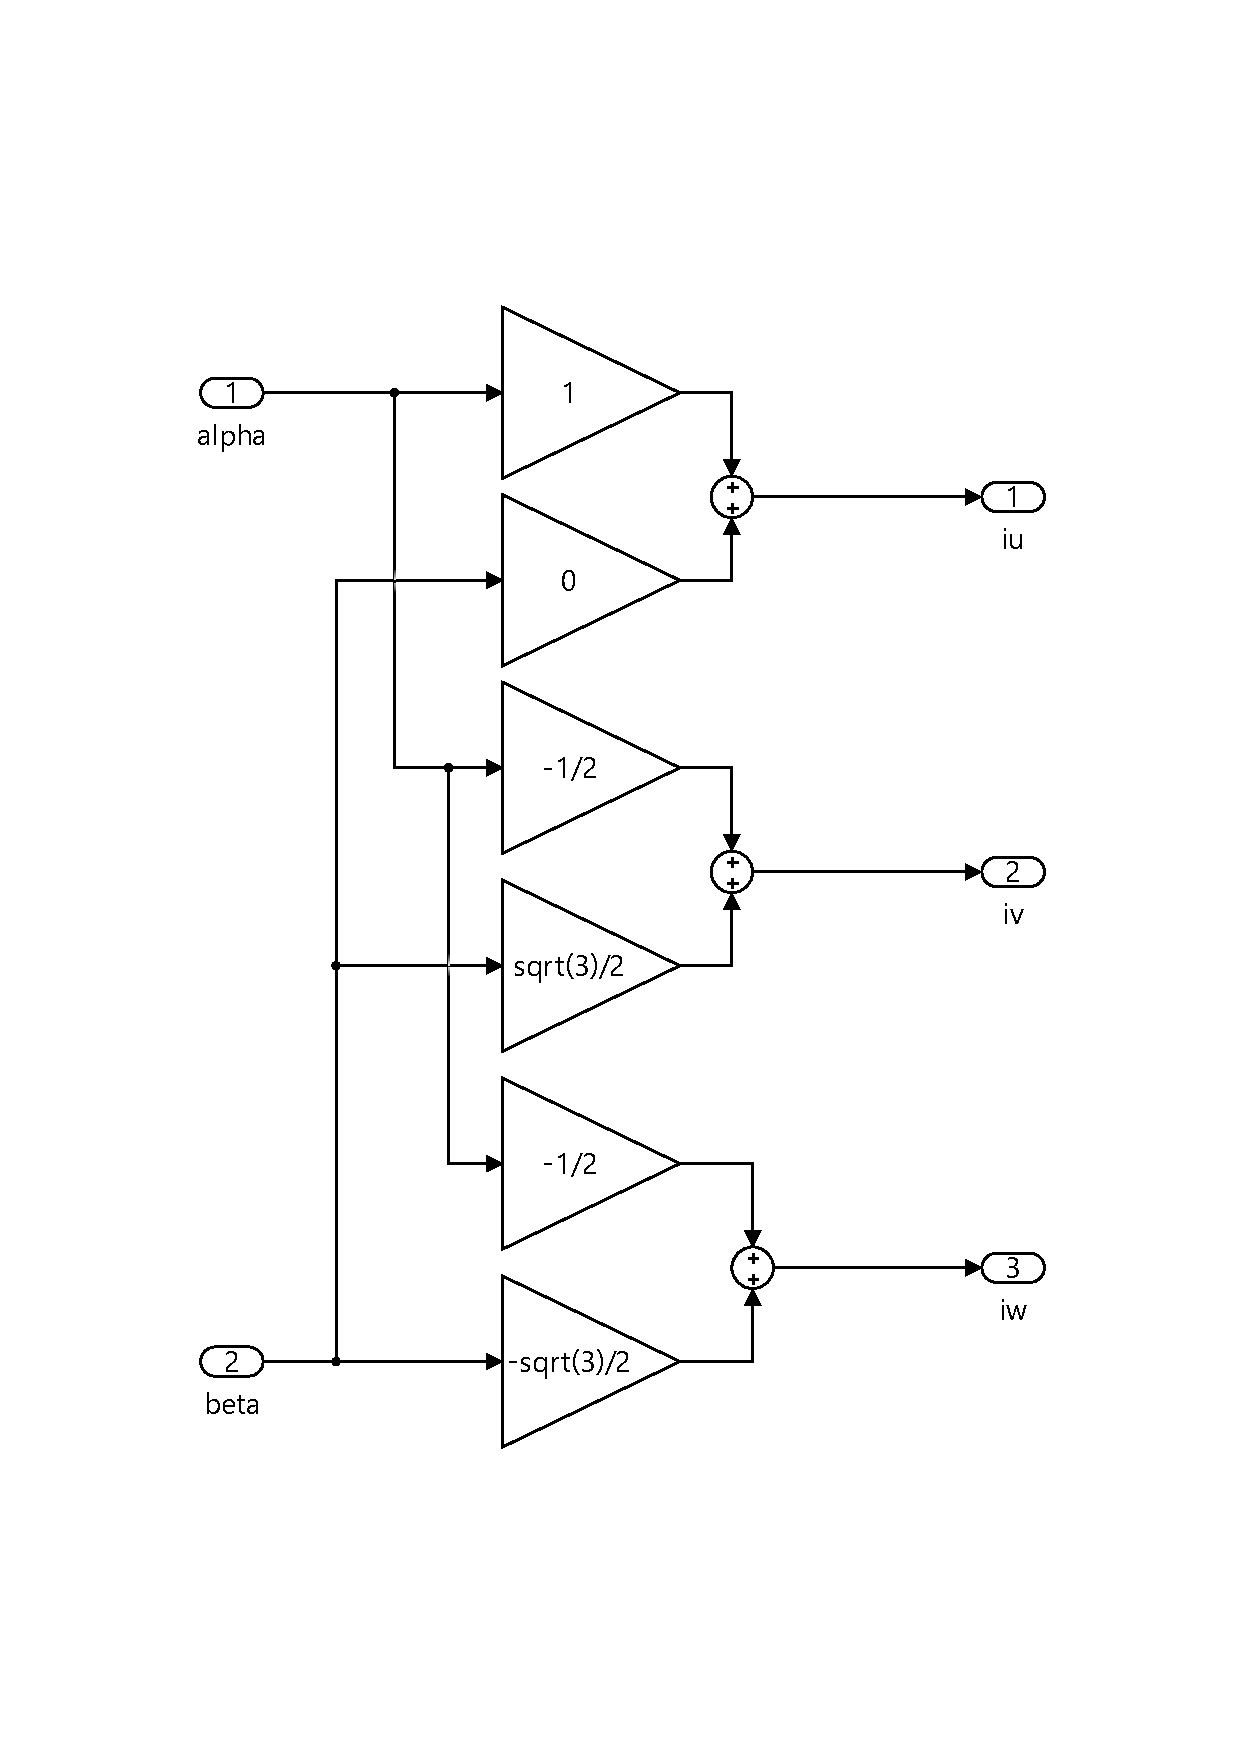
\includegraphics[width=\textwidth]{/simulink/ab_to_uvw.pdf}
%	\label{fig:ab_to_uvw}
%	\caption{Aufbau Inverse Clarke Transformation}
%\end{figure}

Um die Koordinatentransformation zu vervollständigen ist die d-q-, oder Park Transformation, von entscheidender Bedeutung.
Der Block für die d-q-Transformation setzt wird mit dem Zusammenhang \ref{parkvektor} und der Matrix \ref{parkmatrix} erstellt. 
Die inverse d-q-Transformation ist mit Hilfe der Matritzen \ref{parkvektorinvers} sowie \ref{parkmatrixinvers} aufgebaut.

%Die nachstehende Grafik \ref{fig:ab_to_dq} stellt die Park Transformation in Simulink dar:

%\begin{figure}[h]
%	\centering
%	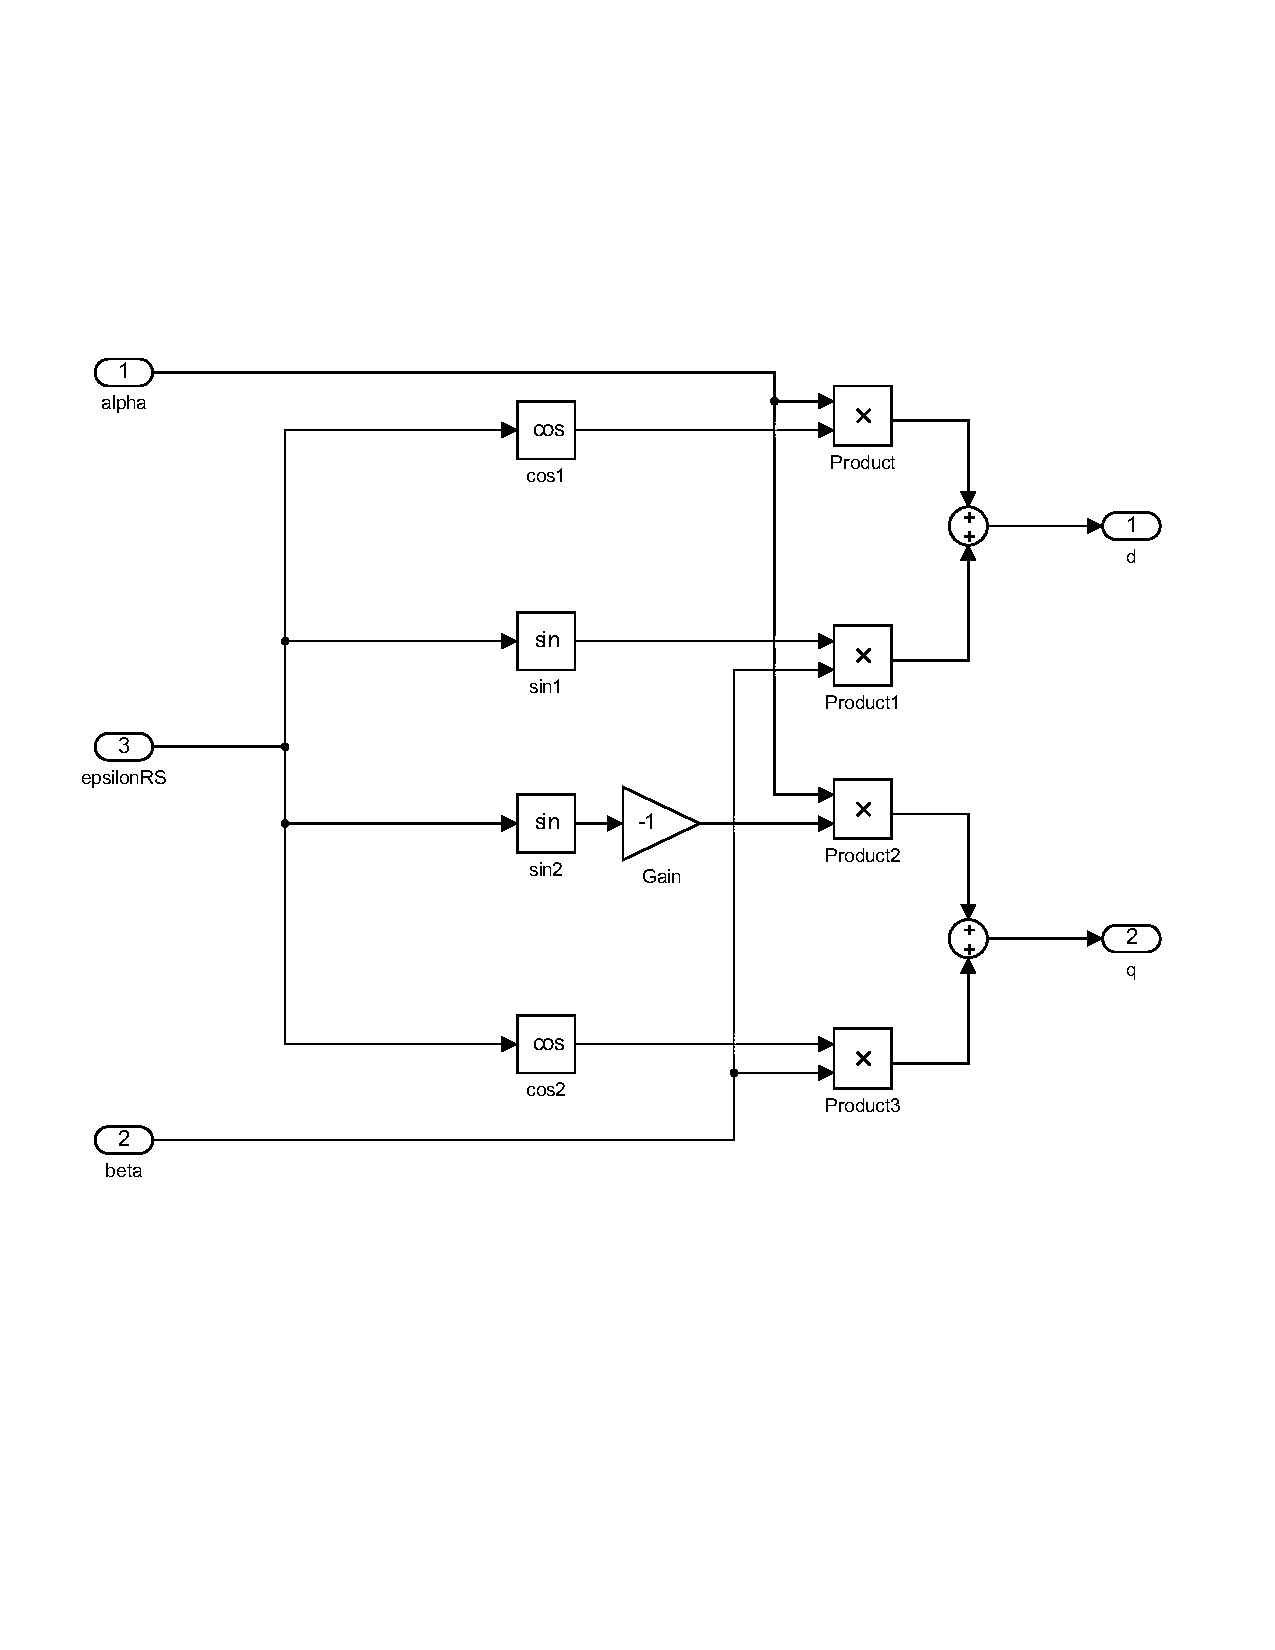
\includegraphics[width=\textwidth]{/simulink/ab_to_dq.pdf}
%	\label{fig:ab_to_dq}
%	\caption{Aufbau Park Transformation}
%\end{figure}

%In Abbildung \ref{fig:dq_to_ab} ist der Aufbau der inversen Park Transformation dargestellt:

%\begin{figure}[h]
%	\centering
%	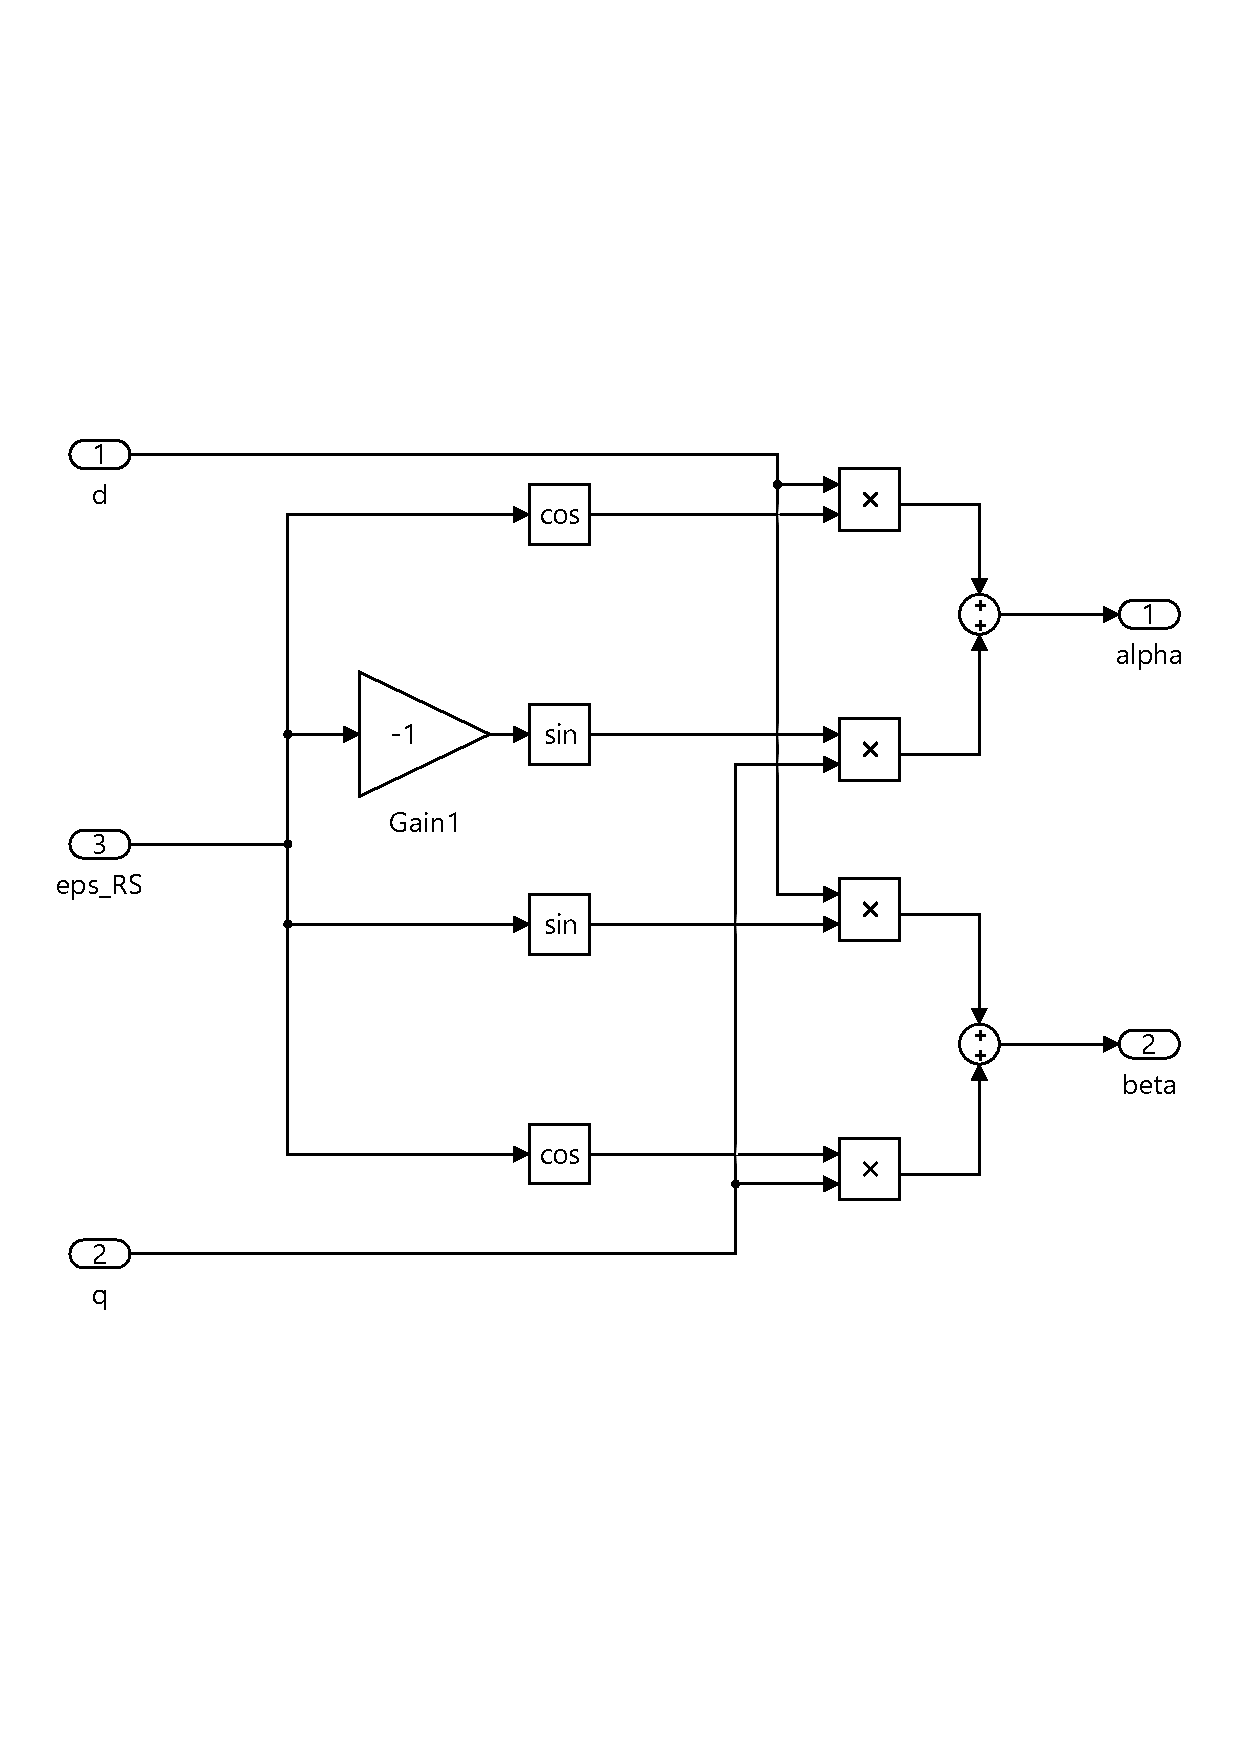
\includegraphics[width=\textwidth]{/simulink/dq_to_ab.pdf}
%	\label{fig:dq_to_ab}
%	\caption{Aufbau Inverse Park Transformation}
%\end{figure}

An dieser Stelle ist es aus übersichtlichkeitsgründen sinnvoll, die Transformationsblöcke als Subsystem zusammenzufassen.
Es ergibt sich für die Clarke-Park Transformation somit ein Block mit drei Eingängen für die drei Wechselgrößen und einem Eingange für $\varepsilon_\i{RS}$, sowie zwei Ausgängen für d- und q-Komponente.
Ebendieses wird auch für die Rücktransformation gemacht. 
Hier ergibt sich ein Subsystem mit drei Eingängen. 
Zwei für d- und q-Größe sowie ebenfalls ein Eingang für $\varepsilon_\i{RS}$.
Es ergeben sich drei Ausgänge für das rückgeführte Dreiphasensystem.

\newpage
\begin{figure}[h]
	\centering
	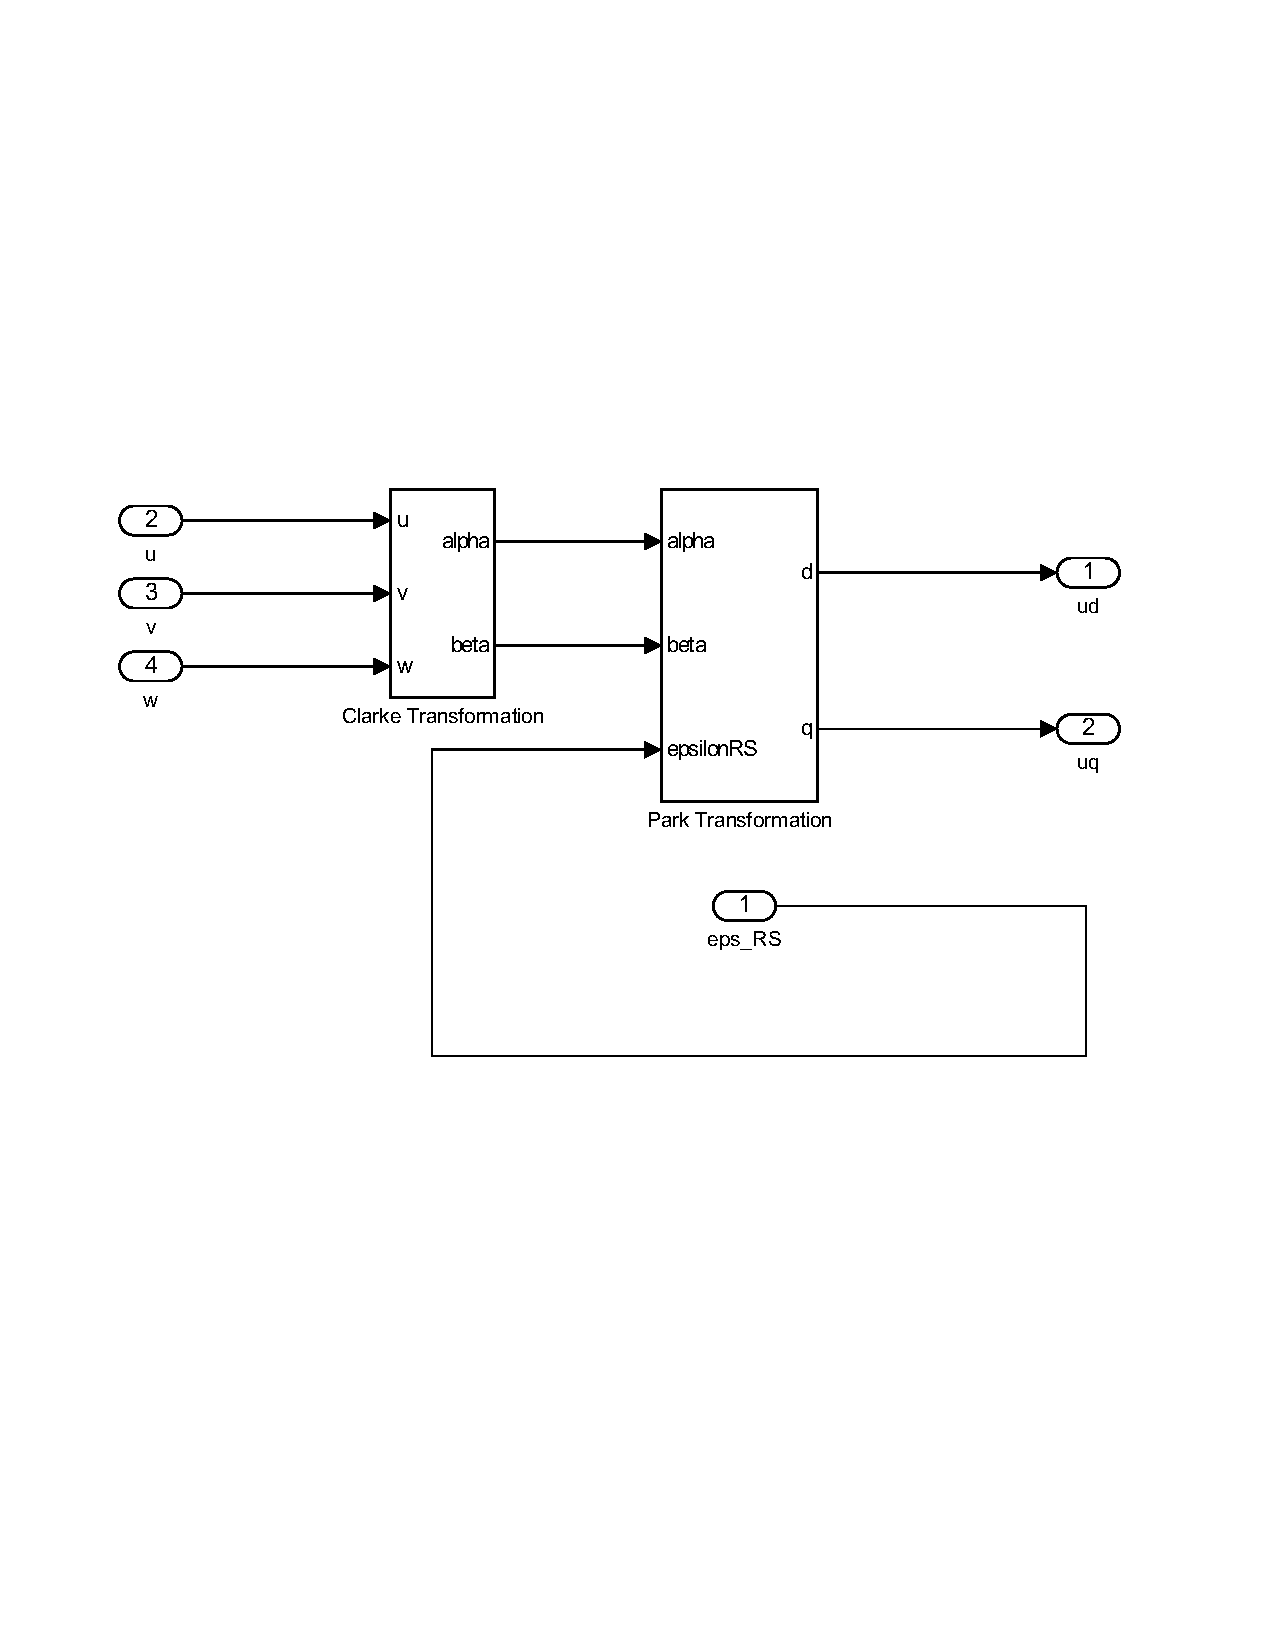
\includegraphics[width=\textwidth]{/simulink/uvw_to_dq.pdf}
	\label{fig:uvw_to_dq}
	\caption{Aufbau Clarke-Park Transformation}
\end{figure}

\begin{figure}[h]
	\centering
	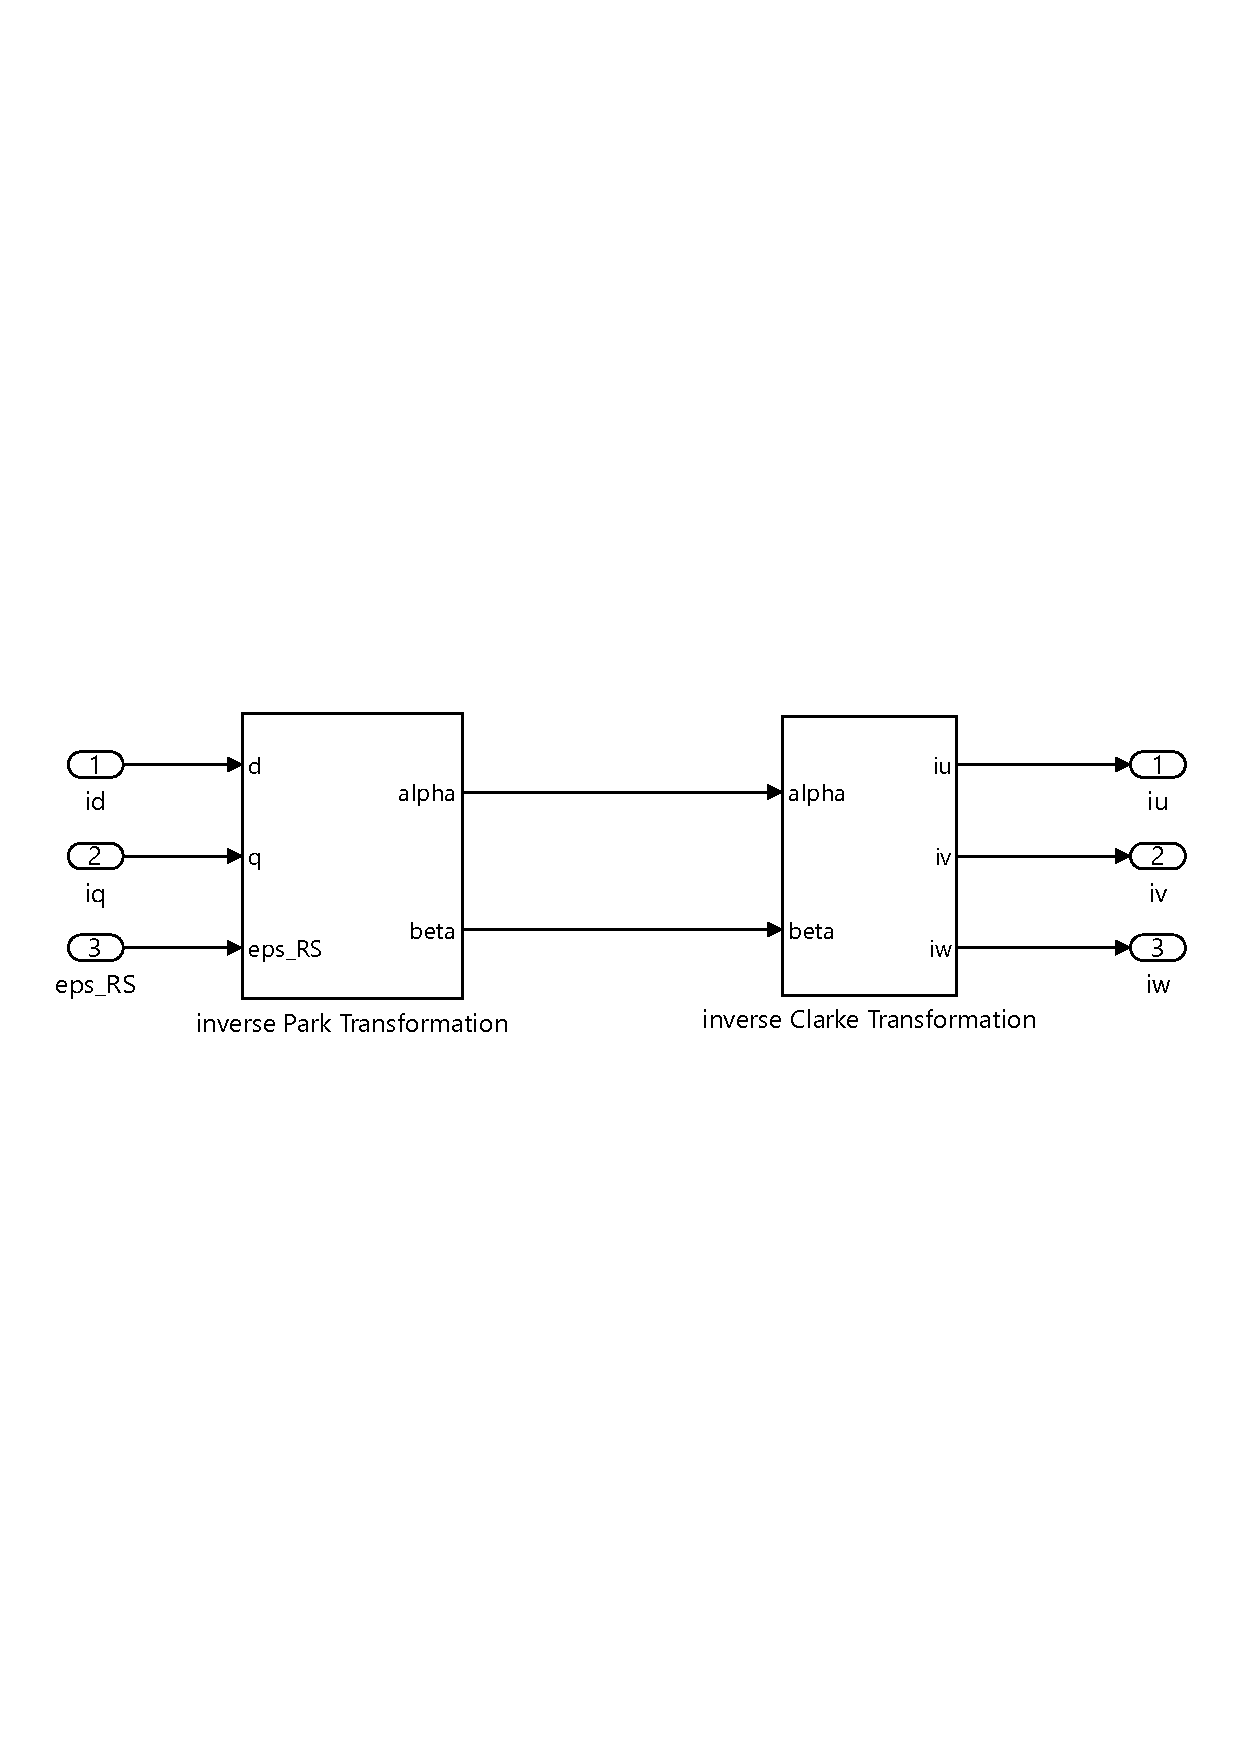
\includegraphics[width=\textwidth]{/simulink/dq_to_uvw.pdf}
	\label{fig:dq_to_uvw}
	\caption{Aufbau inverse Clarke-Park Transformation}
\end{figure}
\newpage

\subsection{Modellierung einer PMSM}

Als Grundlage für die Betrachtung der PMSM gilt der Abschnitt \ref{sec:synchron-dq}.
Die grundlegenden Gleichung dazu sind (\ref{eqn:ud-lin-gleichung}), (\ref{eqn:uq-lin-gleichung}) und (\ref{eqn:mi-lin-gleichung}).
Aus den Gleichungen ergibt sich im Simulink das Modell.
Das Modell wird in zwei Systeme unterteilt:

\begin{itemize}
	\item Mechanical system
	\item Electrical system
\end{itemize}

\begin{figure}[h!]
	\centering
	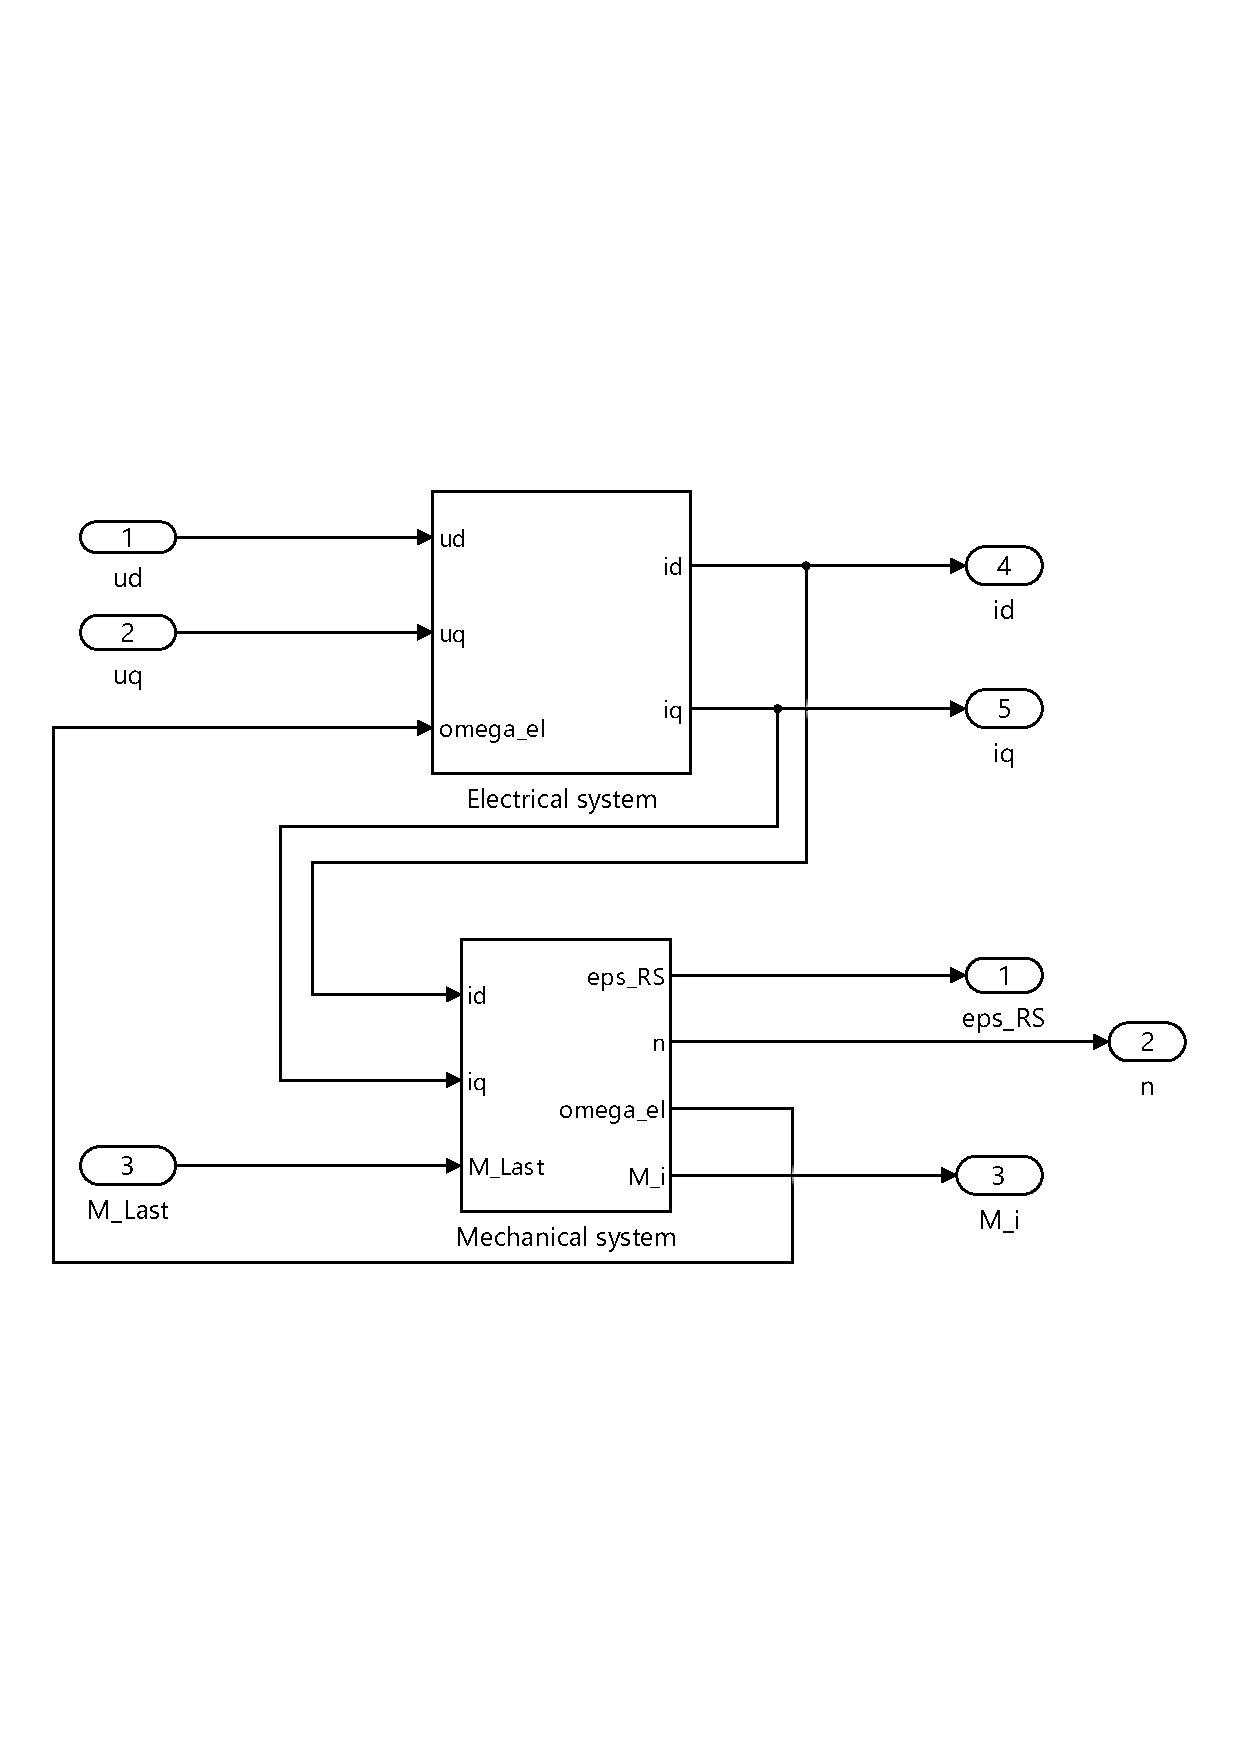
\includegraphics[scale=0.7]{/simulink/pmsm.pdf}
	\label{fig:pmsm}
	\caption{Aufbau des Subsystems: PMSM, mit der Unterteilung in: Electrical system und Mechanical system.}
\end{figure}

Bei dem \enquote{Mechanical system} wird die Differentialgleichung der elektrischen Winkelgeschwindigkeit beschrieben s.~h.~Gl.~(\ref{eqn:mi-lin-gleichung}).
Das \enquote{Electrical system} beschreibt hingegen die Differentialgleichungen der Ströme und somit die elektrischen Parameter einer PMSM.
Die Überführung der Maschinengleichungen erfolgt dabei dem gleichen Prinzip wie in Abschnitt \ref{cha:regelungpmsm}.
Zunächst wird auf das \enquote{Electrical system} eingegangen, welches in Abbildung \ref{fig:electrical-system} dargestellt ist.
Die dabei modellierten Differentialgleichungen~(\ref{eqn:id_dt}) und (\ref{eqn:iq_dt}) werden entsprechend umgesetzt, dabei entsteht das Modell auf Basis eines vereinfachten Modells (s.~h.~Abschnitt~\ref{sec:synchron-dq}~--~Linearisierte Gleichungen (Spannungsgleichungen im rotorfesten System)).
Aus der Bestimmungsgleichung~(\ref{eqn:mi-lin-gleichung}) folgt die elektrische Winkelgeschwindigkeit $\omega_\x{el}$ (s.~h.~Gl.~(\ref{eqn:dw_dt})).

\subsection{Regelblöcke}

Wie im Signalflussplan \ref{fig:signalflussplan} erkennbar, ist zum einen ein Drehzahlregler und zum anderen eine Stromregelung im Modell enthalten. 
Diese dienen dazu, um den Strom entsprechend der Solldrehzahl einzustellen.
Hierzu wurden einfache PI-Regler verwendet.
Die nachstehende Abbildung \ref{fig:drehzahl} zeigt den Aufbau Drehzahlregelung:

\begin{figure}[h]
	\centering
	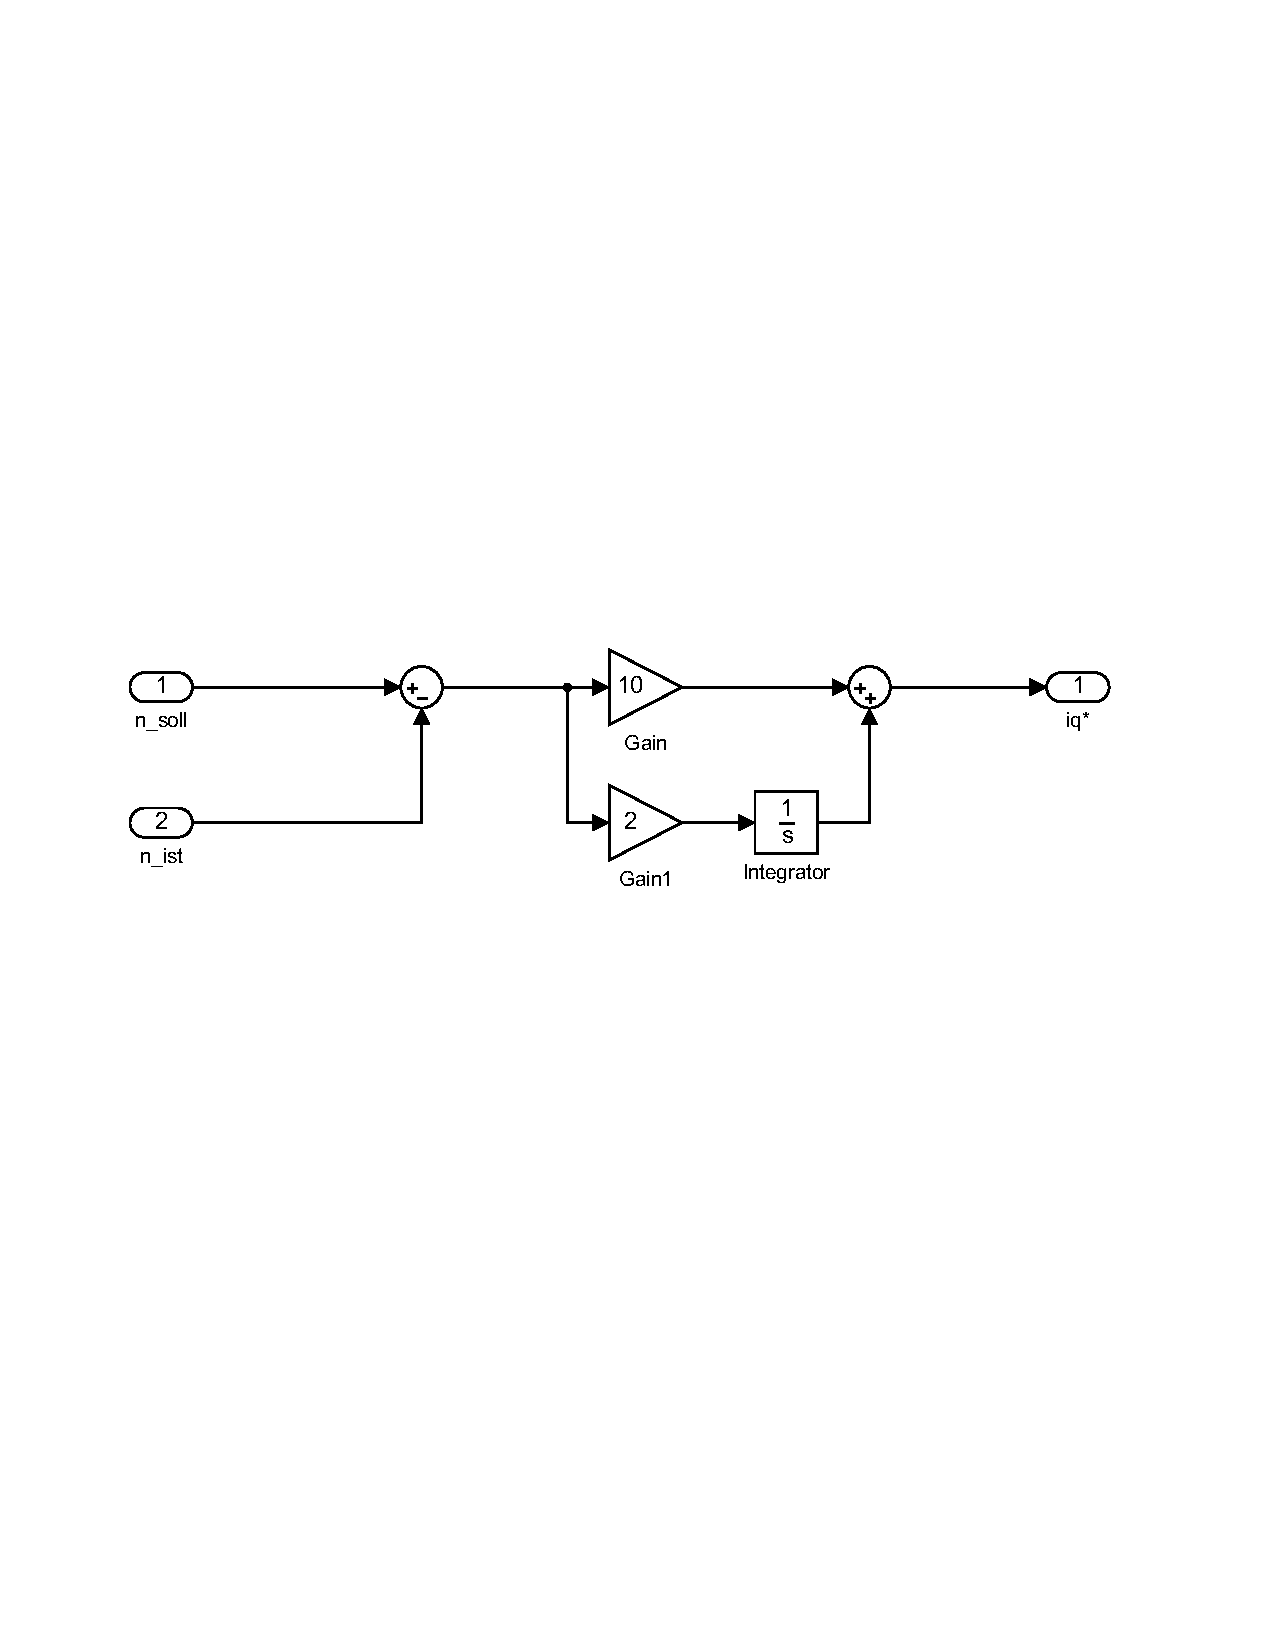
\includegraphics[width=\textwidth]{/simulink/drehzahl.pdf}
	\label{fig:drehzahl}
	\caption{Aufbau der Drehzahlregelung.}
\end{figure}

Der Stromregler wird in Abbildung \ref{fig:stromregelung} gezeigt:

\begin{figure}[h]
	\centering
	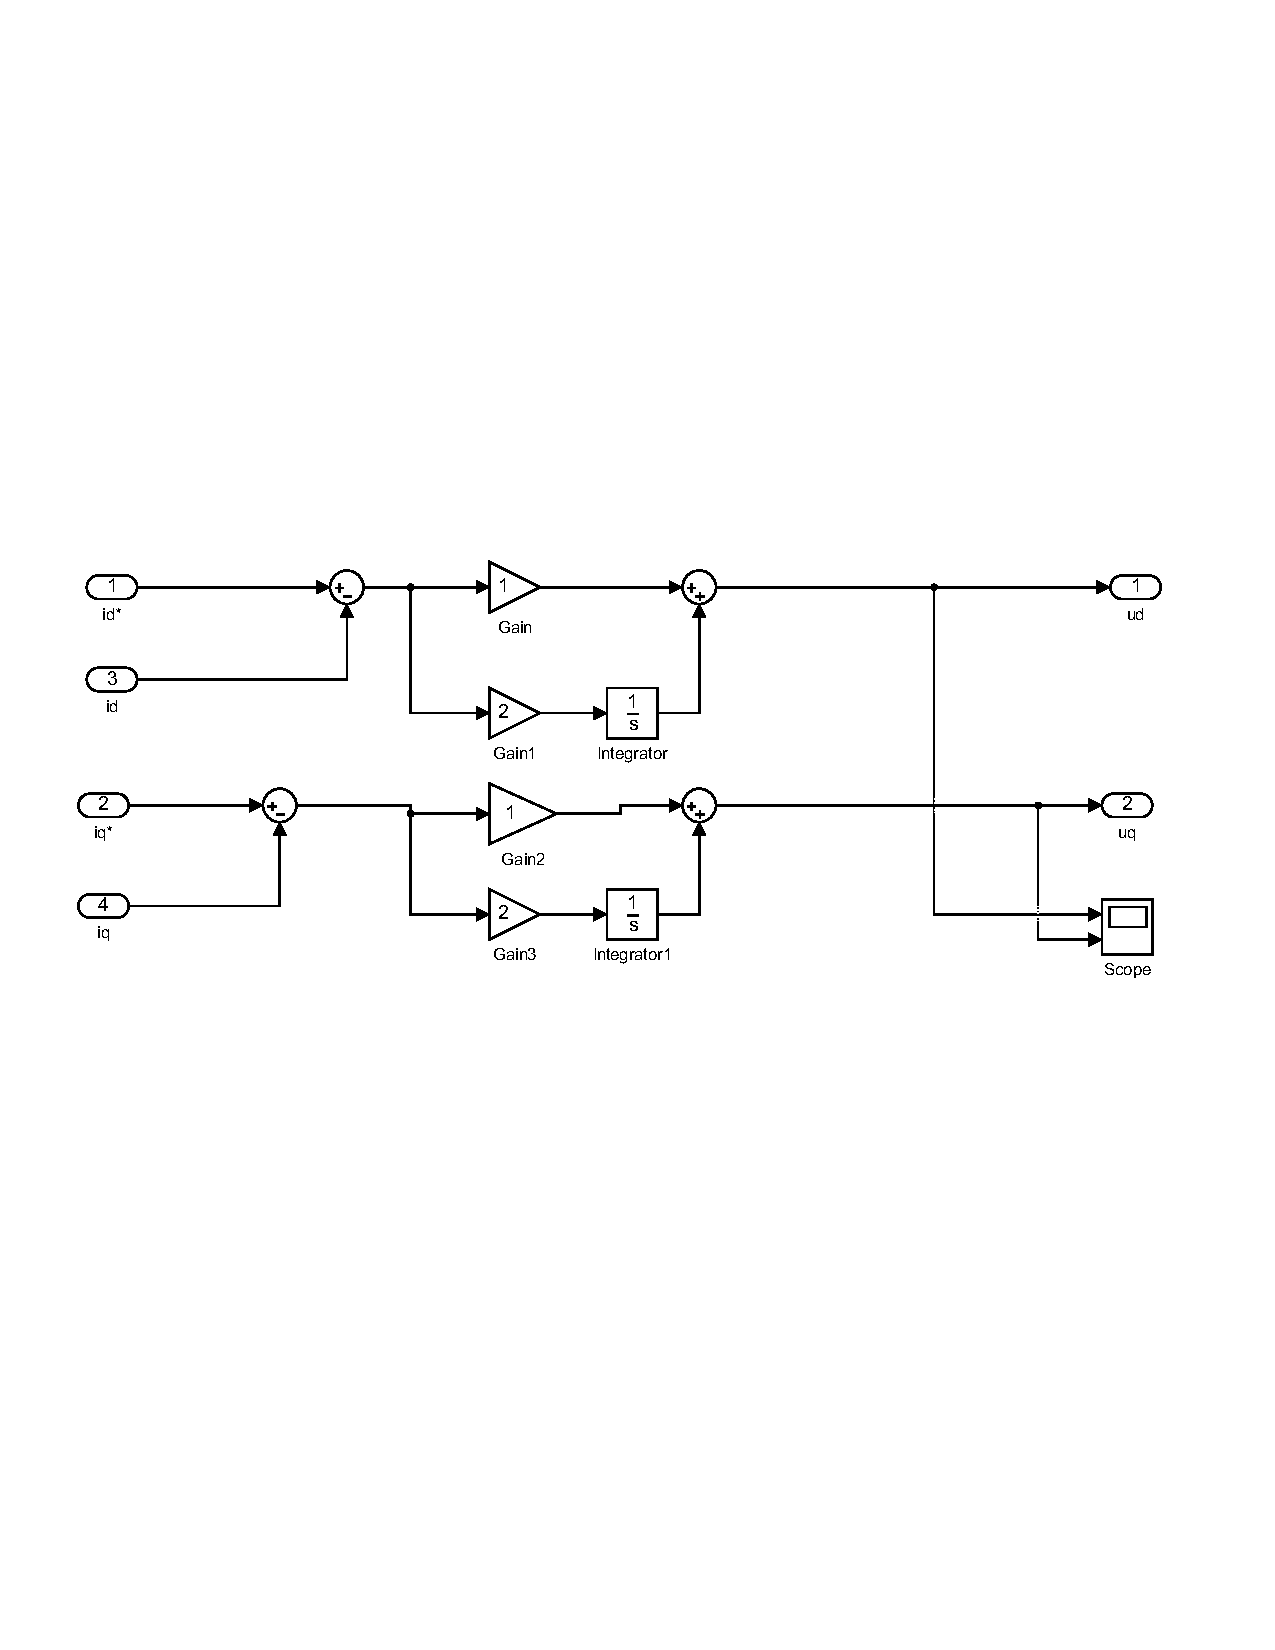
\includegraphics[width=\textwidth]{/simulink/stromregelung.pdf}
	\label{fig:stromregelung}
	\caption{Aufbau der Stromregelung.}
\end{figure}

%%% Local Variables: 
%%% mode: latex
%%% TeX-master: "main"
%%% TeX-open-quote: "\\enquote{"
%%% TeX-close-quote: "}"
%%% LaTeX-csquotes-open-quote: "\\enquote{"
%%% LaTeX-csquotes-close-quote: "}"
%%% End: 
